\title{[Lab2] EEG Classification}
\author{0616014 楊政道}
\maketitle
\thispagestyle{fancy}
\section{Introduction}
\subsection{Lab Objective}
\paragraph{}
In this assignment, I will use pytorch to construct two models, EEGNet and DeepConvNet, with three different activation functions including ReLU, LeakyReLU, and ELU.
\subsection{Dataset}
\paragraph{}
This dataset has two channels. There are 750 data points for each channel. 
\begin{figure}[!ht]
    \begin{center} 
        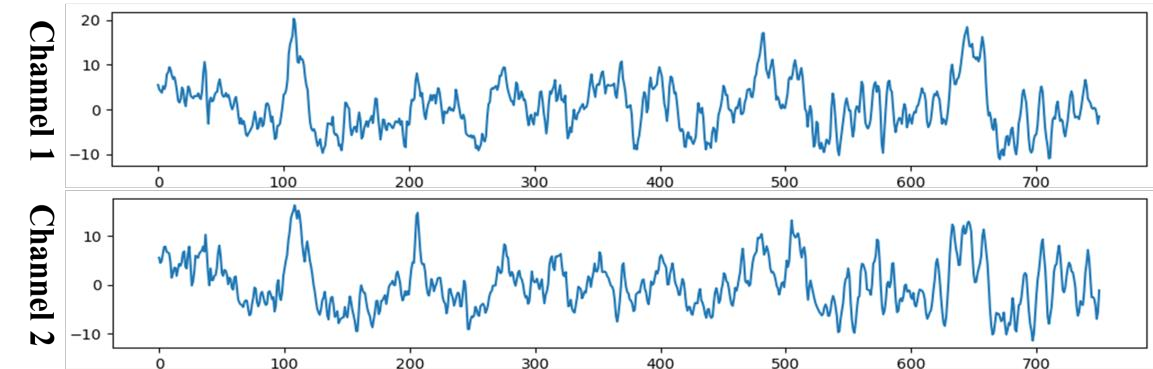
\includegraphics[width=15cm]{eeg.png} 
        \caption{EEG signals}
    \end{center} 
\end{figure}
\subsection{Project Structure}
\dirtree{%
.1 DLP\_LAB2\_0616014\_楊政道.zip.
.2 data/.
.3 dataloader.py.
.2 model/.
.3 DeepConvNet.py.
.3 EEGNet.py.
.2 weight/.
.3 record.json.
.2 train.py.
.2 evaluate.py.
}
\subsubsection{data/dataloader.py}
\paragraph{}
To generate the pytorch dataloader for our training and testing data.
\subsubsection{model/EEGNet.py}
\paragraph{}
To define the structure of EEGNet and its forward function. 
\subsubsection{model/DeepConvNet.py}
\paragraph{}
To define the structure of DeepConvNet and its forward function.
\subsubsection{weight/record.json}
\paragraph{}
To mentain the maximum test accuracy. If we have higher test accuracy, we will replace the weight and update the record file. The model parameters will be stored in weight directory.
\subsubsection{train.py}
\paragraph{}
To define the Trainer class and train networks.
\subsubsection{evaluate.py}
\paragraph{}
It will load the network parameters we have stored and evaluate the network.
\section{Experiment Setup}
\subsection{EEGNet}
\subsubsection{structure}
\begin{lstlisting}[language=Python]
EEGNet(
  (firstconv): Sequential(
    (0): Conv2d(1, 16, kernel_size=(1, 51), stride=(1, 1), padding=(0, 25), bias=False)
    (1): BatchNorm2d(16, eps=1e-05, momentum=0.1, affine=True, track_running_stats=True)
  )
  (depthwiseConv): Sequential(
    (0): Conv2d(16, 32, kernel_size=(2, 1), stride=(1, 1), groups=16, bias=False)
    (1): BatchNorm2d(32, eps=1e-05, momentum=0.1, affine=True, track_running_stats=True)
    (2): [Activation Function]()
    (3): AvgPool2d(kernel_size=(1, 4), stride=(1, 4), padding=0)
    (4): Dropout(p=[dropout], inplace=False)
  )
  (separableConv): Sequential(
    (0): Conv2d(32, 32, kernel_size=(1, 15), stride=(1, 1), padding=(0, 7), bias=False)
    (1): BatchNorm2d(32, eps=1e-05, momentum=0.1, affine=True, track_running_stats=True)
    (2): [Activation Function]()
    (3): AvgPool2d(kernel_size=(1, 8), stride=(1, 8), padding=0)
    (4): Dropout(p=[dropout], inplace=False)
  )
  (classify): Sequential(
    (0): Linear(in_features=736, out_features=2, bias=True)
  )
)
\end{lstlisting}
\subsection{DeepConvNet}
\subsubsection{structure}
\begin{lstlisting}[language=Python]
DeepConvNet(
  (conv0): Sequential(
    (0): Conv2d(1, 25, kernel_size=(1, 5), stride=(1, 1))
    (1): Conv2d(25, 25, kernel_size=(2, 1), stride=(1, 1))
    (2): BatchNorm2d(25, eps=1e-05, momentum=0.1, affine=True, track_running_stats=True)
    (3): [Activation Function]()
    (4): MaxPool2d(kernel_size=(1, 2), stride=(1, 2), padding=0, dilation=1, ceil_mode=False)
    (5): Dropout(p=[dropout], inplace=False)
  )
  (conv1): Sequential(
    (0): Conv2d(25, 50, kernel_size=(1, 5), stride=(1, 1))
    (1): BatchNorm2d(50, eps=1e-05, momentum=0.1, affine=True, track_running_stats=True)
    (2): [Activation Function]()
    (3): MaxPool2d(kernel_size=(1, 2), stride=(1, 2), padding=0, dilation=1, ceil_mode=False)
    (4): Dropout(p=[dropout], inplace=False)
  )
  (conv2): Sequential(
    (0): Conv2d(50, 100, kernel_size=(1, 5), stride=(1, 1))
    (1): BatchNorm2d(100, eps=1e-05, momentum=0.1, affine=True, track_running_stats=True)
    (2): [Activation Function]()
    (3): MaxPool2d(kernel_size=(1, 2), stride=(1, 2), padding=0, dilation=1, ceil_mode=False)
    (4): Dropout(p=[dropout], inplace=False)
  )
  (conv3): Sequential(
    (0): Conv2d(100, 200, kernel_size=(1, 5), stride=(1, 1))
    (1): BatchNorm2d(200, eps=1e-05, momentum=0.1, affine=True, track_running_stats=True)
    (2): [Activation Function]()
    (3): MaxPool2d(kernel_size=(1, 2), stride=(1, 2), padding=0, dilation=1, ceil_mode=False)
    (4): Dropout(p=[dropout], inplace=False)
  )
  (classify): Sequential(
    (0): Linear(in_features=8600, out_features=2, bias=True)
  )
)
\end{lstlisting}
\subsection{Activation Function}
\begin{figure}[!ht]
    \begin{center} 
        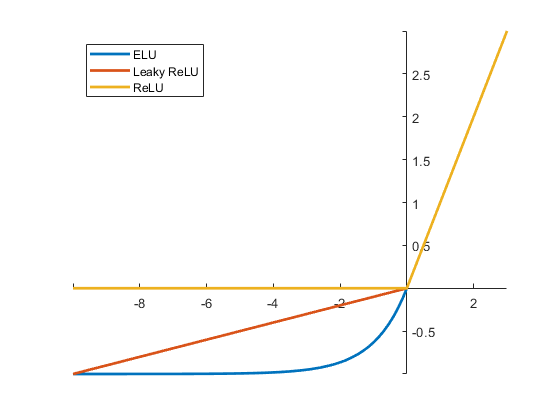
\includegraphics[width=15cm]{activation_function.png} 
        \caption{Activation Function}
    \end{center} 
\end{figure}
\subsubsection{ELU}
$$\texttt{ELU}(x)=\left\{\begin{matrix}
x & x \geq 0\\ 
\alpha (e^x-1) & x < 0
\end{matrix}\right.$$
\subsubsection{ReLU}
$$\texttt{ReLU}(x)=\left\{\begin{matrix}
x & x \geq 0\\ 
0 & x < 0
\end{matrix}\right.$$
\subsubsection{LeakyReLU}
$$\texttt{LeakyReLU}(x)=\left\{\begin{matrix}
x & x \geq 0\\ 
\alpha x & x < 0
\end{matrix}\right.$$
\paragraph{}
The differences of these three activation functions are the part smaller than zero in x. We can find the gradient in ReLU and ELU wiil shrink into zero as the value of the x smaller. It will make gradient shrink when we initialize the network weight too small.
\section{Experimental Result}
\subsection{Comparison Plot}
\subsubsection{EEGNet}
Hyper parameters:
\begin{itemize}
    \item optimizer: Adam
    \item criterion: CrossEntropy
    \item epoch size: 1000
    \item batch size: 1080
    \item learning rate: 0.001
\end{itemize}
\begin{figure}[!ht]
    \begin{center} 
        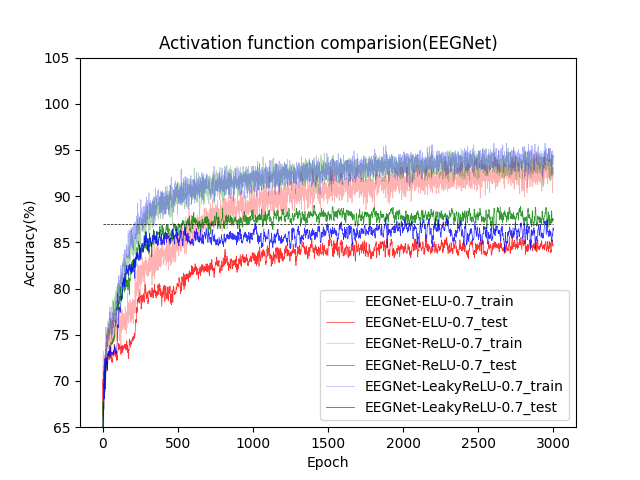
\includegraphics[width=12cm]{eegnet_comparison.png} 
        \caption{EEGNet Comparison}
    \end{center} 
\end{figure}
\subsubsection{DeepConvNet}
\begin{itemize}
    \item optimizer: Adam
    \item criterion: CrossEntropy
    \item epoch size: 3000
    \item batch size: 1080
    \item learning rate: 0.001
\end{itemize}
\begin{figure}[!ht]
    \begin{center} 
        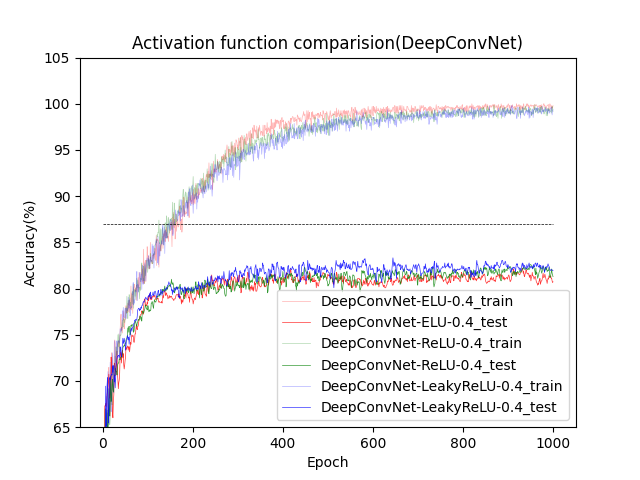
\includegraphics[width=12cm]{deepconvnet_comparison.png} 
        \caption{DeepConvNet Comparison}
    \end{center} 
\end{figure}
\subsection{Highest Test Accuracy}
\subsubsection{EEGNet}
\begin{center}
\begin{tabular}{ |c|c|c||c|  }
\hline
\multicolumn{4}{|c|}{EEGNet} \\
\hline
Model & Acti-Func & Dropout & Max Test Acc\\
\hline
EEGNet & ELU & 0.5 & 85.83\% \\
EEGNet & ELU & 0.6 & 86.76\% \\
EEGNet & ELU & 0.7 & 87.50\% \\
EEGNet & ELU & 0.8 & 82.04\% \\
\hline
EEGNet & LeakyReLU & 0.5 & 87.96\% \\
EEGNet & LeakyReLU & 0.6 & 89.91\% \\
EEGNet & LeakyReLU & 0.7 & 89.62\% \\
EEGNet & LeakyReLU & 0.8 & 86.94\% \\
\hline
EEGNet & ReLU & 0.5 & 88.06\% \\
EEGNet & ReLU & 0.6 & 89.72\% \\
EEGNet & ReLU & 0.7 & \textbf{90.19\%} \\
EEGNet & ReLU & 0.8 & 90.09\% \\
\hline
\end{tabular}
\end{center}
\subsubsection{DeepConvNet}
\begin{center}
\begin{tabular}{ |c|c|c||c|  }
\hline
\multicolumn{4}{|c|}{EEGNet} \\
\hline
Model & Acti-Func & Dropout & Max Test Acc\\
\hline
DeepConvNet & ELU & 0.4 & 83.15\% \\
DeepConvNet & ELU & 0.5 & 83.80\% \\
DeepConvNet & ELU & 0.6 & 82.96\% \\
\hline
DeepConvNet & LeakyReLU & 0.4 & \textbf{86.02\%} \\
DeepConvNet & LeakyReLU & 0.5 & 85.56\% \\
DeepConvNet & LeakyReLU & 0.6 & 84.26\% \\
\hline
DeepConvNet & ReLU & 0.4 & 85.83\% \\
DeepConvNet & ReLU & 0.5 & 84.35\% \\
DeepConvNet & ReLU & 0.6 & 82.50\% \\
\hline
\end{tabular}
\end{center}
\section{Discussion}
\subsection{Dropout}
\begin{figure}[!ht]
    \begin{center} 
        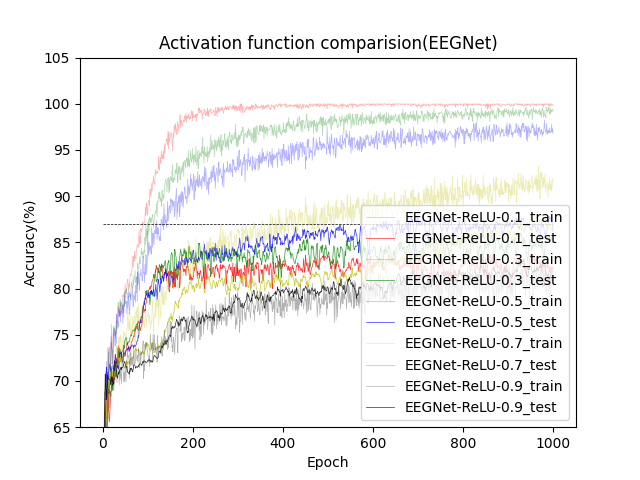
\includegraphics[width=15cm]{dropout.png} 
        \caption{EEGNet vs Dropout}
    \end{center} 
\end{figure}
\paragraph{}
If we set the dropout rate too low(red line), the training accuracy will increase fast but testing accuracy still remains low. The model will be overfitting and perform bad on the test dataset.
\paragraph{}
On the other hand, if we set the dropout rate too high(black line), the training accuracy can't increase and the network will learning nothing. The testing accuracy, of course, will still remain low. The model will be underfitting and perform bad on the test dataset too.
\paragraph{}
Therefore, it's important to tune the dropout rate in order to prevent the model from overfitting and underfitting.
